%====================================================
%	CHAPTER 5 - Allocation
%====================================================
\chapter{Controller Allocation}
\label{ch:allocation}
%====================================================
Static allocation rules are now developed which aim to solve for actuator commands calculated from a given control input, neither adaptive nor online allocation rules are considered here. Static allocation neglects to account for individual actuator dynamics and transfer rates. Such effects are assumed to be accounted for by the major loop control coefficients, described in Ch:\ref{ch:control}, when optimized subsequently in Sec:\ref{sec:simulation.tuning}.
\par
Higher level attitude and position controllers (from Sec:\ref{sec:control.attitude} and Sec:\ref{sec:control.position} respectively) design a virtual control input $\mathcal{H}(\vec{\mathbf{x}}_e,t)=\vec{\nu}_d=[\vec{F}_d~\vec{\tau}_d]^T$ to be applied by the vehicle's actuator plant. The vehicle's mechanical overactuation was described in Sec:\ref{sec:control.inputs} but a simplified allocation block, reduced from control loop diagram in Fig:\ref{fig:control-block}, is illustrated in Fig:\ref{fig:allocation-block}.
\begin{figure}[htbp]
\vspace{-6pt}
\centering
\begin{subfigure}{0.48\textwidth}
\centering
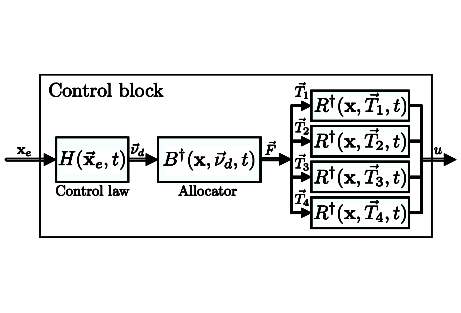
\includegraphics[width=\textwidth]{figs/allocator-block}
\vspace{-12pt}
\caption{Allocation block}
\label{fig:allocation-block}
\end{subfigure}
\begin{subfigure}{0.48\textwidth}
\centering
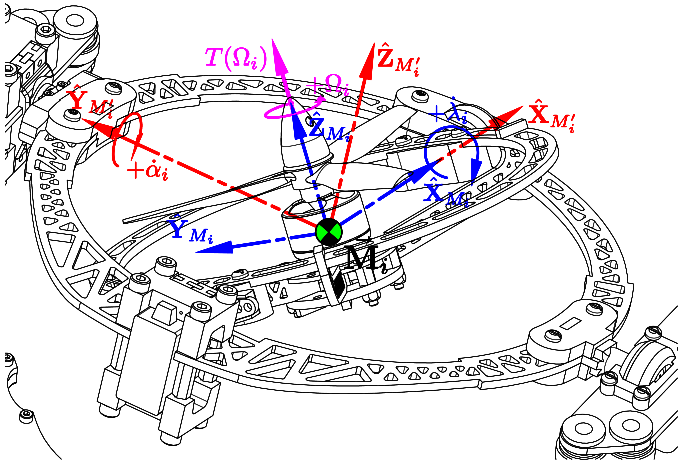
\includegraphics[width=\textwidth]{figs/force-redirect}
\vspace{-12pt}
\caption{Single thrust vector construction}
\label{fig:allocation-redirect}
\end{subfigure}
\vspace{-6pt}
\caption{Actuator allocation}
\vspace{-18pt}
\end{figure}
\par
Some distribution heuristic is needed to \emph{allocate} physical actuator positions $\vec{u}_c\in\mathbb{U}$ that command the control input $\vec{\nu}_c$, from Eq:\ref{eq:control-input}. As mentioned previously (pseudo) inversion based allocation uses an affine actuator effectiveness function, however it is worth mentioning a multiplicative effectiveness function is \emph{convenient} but not crucial to allocation. The allocator is abstracted to first solve for four thrust vectors which are applied by each motor module, Eq:\ref{eq:4.7}. As per convention $B^\dagger$ represents the pseudo inverse of the allocator's effectiveness function $B$:
\begin{equation}\label{eq:5.1}
\vec{T}_{[1:4]}=B^{\dagger}(\vec{\mathbf{x}},t)\vec{\nu}_d=\begin{bmatrix}
\vec{T}_1&\vec{T}_2&\vec{T}_3&\vec{T}_4
\end{bmatrix}^T~~~~\in\mathbb{R}^{1\times 12}
\end{equation}
Each 3-D thrust vector is then used to solve for each module's propeller speed in $[\text{RPM}]$ and both servo rotational positions in $[\text{rad}]$, undoing the thrust vectoring (rotation) applied by the motor module's actuator structure in Fig:\ref{fig:allocation-redirect}.
\begin{equation}
u_i = \begin{bmatrix}\Omega_i&\lambda_i&\alpha_i\end{bmatrix}^T=R^\dagger(\vec{\mathbf{x}},\vec{T}_i,t)~~~~\text{for}~i\in[1:4]
\end{equation}
%====================================================
\section{Generalized allocation}
\label{sec:allocation.slack}
%====================================================
Regular, unconstrained control allocation is solved as an optimization problem, shown in \cite{allocation,controlallocation}. The aim is to minimize deviation (\emph{slack}) $\vec{s}$ between the virtual controller generated input  $\vec{\nu}_d$ and the physically commanded control input $\vec{\nu}_c(u_c)$, where $u_c$ is a commanded actuator position. For a controller's virtual input $\vec{\nu}_d=\mathcal{H}(\vec{\mathbf{x}}_e,t)$, the problem is to optimize some cost function of the slack variable $Q(\vec{s}\hspace{2pt})$:
\begin{subequations}\label{eq:allocation-slack}
\begin{equation}\label{eq:allocation-slack.a}
\vec{s}\triangleq \vec{\nu}_d-\vec{\nu}_c(\vec{u}_c)
\end{equation}
\vspace{-14pt}
\begin{equation}\label{eq:allocation-slack.b}
\underset{\vec{u}_c\in\mathbb{U}^{m},~\vec{s}\in\mathbb{R}^{n}}{min}\big(Q(\vec{s}\hspace{2pt})\big)~~\text{such that}~~\vec{s}=\mathcal{H}(\vec{\mathbf{x}}_e,t)-B(\vec{\mathbf{x}},t,\vec{u}_c)
\end{equation}
\end{subequations}
where $\vec{u}_c\in\mathbb{U}^m$ is the dimension of the actuator set and $\vec{\mathbf{x}},~\vec{\nu}_d,~\vec{\nu}_c$ and $\vec{s}$ are each the same dimension as the virtual plant's input $\in\mathbb{R}^{n}$, where $n$ is the state's degree of freedom. In this case $u\in\mathbb{U}^{12}$ for the twelve actuators and $\vec{\mathbf{x}}\in\mathbb{R}^6$ for the 6-DOF rigid body. Typically the slack cost function $Q(\vec{s}\hspace{2pt})$ in Eq:\ref{eq:allocation-slack.b} is simply the Euclidean norm of $\vec{s}$:
\begin{equation} 
Q(\vec{s}\hspace{2pt})\triangleq||\vec{s}\hspace{2pt}||=||\vec{\nu}_d-\vec{\nu}_c(\vec{u}_c)||
\end{equation}
Overactuation implies that there exists an entire set of suitable actuator values which are all solutions to Eq:\ref{eq:allocation-slack}. Solving for explicit actuator positions requires an introduction of a secondary cost function or minimization objective $J(\vec{\mathbf{x}},\vec{u}_c,t)$ to refine the solution to Eq:\ref{eq:allocation-slack}.
\begin{equation}\label{eq:allocation-problem}
\underset{\vec{u}\in\mathbb{U}^{12},~\vec{s}\in\mathbb{R}^{6}}{min}\big(||\vec{s}\hspace{2pt}||+J(\vec{\mathbf{x}},\vec{u}_c,t)\big)~~\text{such that}~~\vec{s}=\vec{\nu}_d-\vec{\nu}_c(\vec{u}_c)
\end{equation}
That secondary cost $J(\vec{\mathbf{x}},\vec{u}_c,t)$ and how to calculate its \emph{explicit} minimization solution for Eq:\ref{eq:allocation-problem} is the subject of control allocation. Not much work has been done on overallocation for aerospace vehicles outside the field of satellite attitude control (Sec:\ref{subsubsec:intro.lit.control.allocation} for examples). Often satellites are overactuated for the sake of fault tolerance and redundancy\cite{FTCallocation,discreteFTC}. 
\par
Allocation \emph{inverts} the effectiveness of the actuator set, $B(\vec{\mathbf{x}},u,t)$ in Eq:\ref{eq:control-effectiveness}, to find actuator positions which satisfy the virtual control input. Using pseudo-inversion to solve for an actuator command requires an affine relationship between the effectiveness function and the actuator input matrix $\vec{u}$, hence the abstraction layer which was introduced previously in Eq:\ref{eq:4.7}. The allocator effectiveness function, when abstracted to an affine matrix, reduces to:
\begin{subequations}\label{eq:5.6}
\begin{equation}
\vec{\nu}_d=\mathcal{H}(\vec{\mathbf{x}}_e,t)
\end{equation}
\vspace{-18pt}
\begin{equation}
\vec{\nu}_c(\vec{u}_c)=B(\vec{\mathbf{x}},\vec{u}_c,t)=B'(\vec{\mathbf{x}},t)\vec{u}_c=\begin{bmatrix}
\vec{F}_c(\hat{u}_c)&
\vec{\tau}_c(\hat{u}_c)^T
\end{bmatrix}
\end{equation}
\end{subequations}
where $\vec{F}_c(\hat{u}_c)$ and $\vec{\tau}_c(\hat{u}_c)$ are the physically allocated force and torque acting on the body as a result of the commanded actuator matrix \emph{estimate} $\hat{u}_c$. The allocator solves for an actuator command setpoint $\vec{u}_c$ which leads to actuator response estimate $\hat{u}_c=C(s)\vec{u}_c$ from the actuator block transfer function defined in Eq:\ref{eq:actuator-constraints}. In Eq:\ref{eq:5.6} state dimensions are such that $(\vec{\nu}_d,\vec{\nu}_c)\in\mathbb{R}^n,\vec{u}_c\in\mathbb{U}\in\mathbb{R}^m,~\text{and}~B\in\mathbb{R}^{m\times n}$. The introduced affine abstraction $B'(\vec{\mathbf{x}},t)u_c$ in Eq:\ref{eq:4.7} makes addressing the allocation conceptually simpler, accommodating the use of inversion based allocation laws (Sec:\ref{subsec:allocation.allocators.inverse}-\ref{subsec:allocation.allocators.weightedinverse}).
%====================================================
\section{Thrust vector inversion}
\label{sec:allocation.inversion}
%====================================================
The rotation \emph{inversion} function $R^\dagger(\vec{\mathbf{x}},\vec{F}_i,t)$ to solve for physical actuator positions to be commanded $\vec{u}_c(i)=[\Omega_i~\lambda_i~\alpha_i]^T$ is as yet undefined. Assume for now there is some allocation rule that, from the controller input $\vec{\nu}_d$, designs four decomposed 3-D thrust vectors $\vec{T}_{[1:4]}$ to be actuated by each motor module. 
\par
It then follows that each of those four thrust vectors relate to their individual associated motor module actuator positions through a quaternion \emph{rotation}, not transformation:
\begin{subequations}
\begin{equation}\label{eq:quaternion-thrust-allocation}
\vec{T}_i= Q_{M_i}\otimes\vec{T}(\Omega_i)\otimes Q_{M_i}^*~~~~\in\mathcal{F}^b
\end{equation}
\vspace{-16pt}
\begin{equation}\label{eq:quaternion-thrust-allocation-expanded}
=Q_{z}(\sigma_i)Q_{y}(\alpha_i)Q_{x}(\lambda_i)\otimes \vec{T}(\Omega_i) \otimes Q_{x}^*(\lambda_i)Q_{y}^*(\alpha_i)Q_z^*(\sigma_i)
\end{equation}
Where each motor's thrust vector $\vec{T}(\Omega_i)$ is calculated using blade element momentum theory thrust coefficients, Eq:\ref{eq:thrust-coefficient} with coefficients from Fig:\ref{fig:coeffs-plot}. A propeller's produced thrust is normal to its rotational plane, so in the motor module $\vec{T}(\Omega_i)$ acts in the $\hat{Z}_{M_i}$ direction of that module's frame $\mathcal{F}^{M_i}$:
\begin{equation}
\vec{T}(\Omega_i)=\begin{bmatrix}
0&
0&
T(\Omega_i)
\end{bmatrix}^T=\begin{bmatrix}
0\\
0\\
C_T(J)\rho \Omega_i^2 D^4
\end{bmatrix}~~~~\in\mathcal{F}^{M_i}
\end{equation}
\end{subequations}
Noting that quaternion rotation (or \emph{transformation}) operators change the reference frame but retain the vector operand's magnitude, it follows that $T(\Omega_i)$, and by extension the propeller speed $\Omega_i$, can be found:
\begin{subequations}\label{eq:5.8}
\begin{equation}
|\vec{T}_i|=\sqrt{\norm{\begin{bmatrix}T_x&T_y&T_z\end{bmatrix}}}=\sqrt{T_x^2+T_y^2+T_z^2}=|T(\Omega_i)|=|C_T(J)\rho\Omega_i^2D^4|
\end{equation}
\vspace{-14pt}
\begin{equation}
\therefore\Omega_i=\sqrt{\frac{|\vec{T}_i|}{C_T(J)\rho D^4}}=\sqrt{\frac{\sqrt{T_x^2+T_y^2+T_z^2}}{C_T(J)\rho D^4}}
\end{equation}
\end{subequations}
Reversing (or \emph{undoing}) that transformation from the motor module's frame to the body frame in Eq:\ref{eq:quaternion-thrust-allocation}:
\begin{subequations}
\begin{equation}
\vec{T}(\Omega_i)=Q_{z}^*(\sigma_i)Q_{y}^*(\alpha_i)Q_{x}^*(\lambda_i)\otimes \vec{T}_i \otimes Q_{x}(\lambda_i)Q_{y}(\alpha_i)Q_z(\sigma_i)~~~~\in\mathcal{F}^{M_i}
\end{equation}
\vspace{-14pt}
\begin{equation}\label{eq:thrust-vector-motor-transformation}
\therefore\vec{T}(\Omega_i)=Q_{M_i}^*\otimes \vec{T}_i \otimes Q_{M_i}~~~~\in\mathcal{F}^{M_i}
\end{equation}
\end{subequations}
Knowing only $\vec{T}(\Omega_i)$ and $\vec{T}_i$ in the motor frame and body frame respectively requires solving for a quaternion which relates the two. If both vectors are of unit length, $\breve{T}_i$ and $\breve{T}(\Omega_i)$, then the following relationship can be used to construct a relative quaternion, \cite{rotationsequences}.
\begin{subequations}
\begin{equation}
\breve{T}_i\triangleq\frac{\vec{T}_i}{|\vec{T}_i|}=\frac{\vec{T}_i}{\sqrt{T_x^2+T_y^2+T_z^2}}~~~~\in\mathcal{F}^b
\end{equation}
\vspace{-8pt}
\begin{equation}
\breve{T}(\Omega_i)\triangleq\frac{\vec{T}(\Omega_i)}{|\vec{T}(\Omega_i)|}=\frac{\vec{T}(\Omega_i)}{|C_T(J)\rho\Omega^2 D^4|}=\begin{bmatrix}
0 & 0 & 1
\end{bmatrix}^T~~~~\in\mathcal{F}^{M_i}
\end{equation}
\vspace{-4pt}
\begin{equation}\label{eq:vector-quaternion}
\therefore Q_{M_i}=\begin{bmatrix}
q_0\\
\vec{q}
\end{bmatrix}
=
\begin{bmatrix}
1+\breve{T}_i\cdot \breve{T}(\Omega_i)\\
-\breve{T}_i\times\breve{T}(\Omega_i)
\end{bmatrix}
\end{equation}
\end{subequations}
where Eq:\ref{eq:vector-quaternion} is a quaternion operator's definition Eq:\ref{eq:quaternion-operator}, rotating a vector around a single Euler axis, Eq:\ref{eq:quaternion-euler-axis}, but when applied to two unit vectors. That quaternion can indeed be used to solve for relative pitch, roll and yaw Euler angles (see App:\ref{app:equations.quaternions}). However, Eq:\ref{eq:vector-quaternion} solves for the \textbf{shortest rotational path} between the two vectors, a sequenced ZYX rotation is by no means the shortest possible rotation. Associated $[\phi,~\theta,~\psi]^T$ solutions to Eq:\ref{eq:app-quaternion-eule} are of no consequence when solving for the sequentially applied rotation angles $[\lambda_i,~\alpha_i,~\sigma_i]^T$, where $\sigma_i$ is a known orthogonal multiplicate. Furthermore, when considering a sequenced ZYX quaternion, angular operands cannot be extracted without applying significantly complex trigonometric inversions:
\begin{subequations}
\begin{equation}
Q_b\triangleq\begin{bmatrix}
cos\frac{\psi}{2}\\
0\\
0\\
sin\frac{\psi}{2}
\end{bmatrix}
\otimes
\begin{bmatrix}
cos\frac{\theta}{2}\\
0\\
sin\frac{\theta}{2}\\
0
\end{bmatrix}
\otimes
\begin{bmatrix}
cos\frac{\phi}{2}\\
sin\frac{\phi}{2}\\
0\\
0
\end{bmatrix}
=
\begin{bmatrix}
c\frac{\psi}{2}c\frac{\theta}{2}c\frac{\phi}{2}+s\frac{\psi}{2}s\frac{\theta}{2}s\frac{\phi}{2}\\
c\frac{\psi}{2}c\frac{\theta}{2}s\frac{\phi}{2}-s\frac{\psi}{2}s\frac{\theta}{2}c\frac{\phi}{2}\\
c\frac{\psi}{2}s\frac{\theta}{2}c\frac{\phi}{2}+s\frac{\psi}{2}c\frac{\theta}{2}s\frac{\phi}{2}\\
s\frac{\psi}{2}c\frac{\theta}{2}c\frac{\phi}{2}-c\frac{\psi}{2}s\frac{\theta}{2}s\frac{\phi}{2}
\end{bmatrix}
=
\begin{bmatrix}
q_0\\
q_x\\
q_y\\
q_z
\end{bmatrix}
=
\begin{bmatrix}
q_0\\
\vec{q}
\end{bmatrix}
\end{equation}
\vspace{-4pt}
\begin{equation}
=
\begin{bmatrix}
c\frac{\psi}{2}c\frac{\theta}{2}c\frac{\phi}{2}+s\frac{\psi}{2}s\frac{\theta}{2}s\frac{\phi}{2}\\
c\frac{\psi}{2}c\frac{\theta}{2}s\frac{\phi}{2}-s\frac{\psi}{2}s\frac{\theta}{2}c\frac{\phi}{2}\\
c\frac{\psi}{2}s\frac{\theta}{2}c\frac{\phi}{2}+s\frac{\psi}{2}c\frac{\theta}{2}s\frac{\phi}{2}\\
s\frac{\psi}{2}c\frac{\theta}{2}c\frac{\phi}{2}-c\frac{\psi}{2}s\frac{\theta}{2}s\frac{\phi}{2}
\end{bmatrix}
\otimes
\vec{T}(\Omega_i)
\otimes
\begin{bmatrix}
s\frac{\psi}{2}s\frac{\theta}{2}s\frac{\phi}{2}+c\frac{\psi}{2}c\frac{\theta}{2}c\frac{\phi}{2}\\
s\frac{\psi}{2}s\frac{\theta}{2}c\frac{\phi}{2}-c\frac{\psi}{2}c\frac{\theta}{2}s\frac{\phi}{2}\\
-c\frac{\psi}{2}s\frac{\theta}{2}c\frac{\phi}{2}-s\frac{\psi}{2}c\frac{\theta}{2}s\frac{\phi}{2}\\
c\frac{\psi}{2}s\frac{\theta}{2}s\frac{\phi}{2}-s\frac{\psi}{2}c\frac{\theta}{2}c\frac{\phi}{2}
\end{bmatrix}
\end{equation}
\end{subequations}
Instead, return to rotation matrices to resolve the inverse transformation and note that Euler angle equivalents for the servos are $[\phi,~\theta,~\psi]^T\iff [\lambda_i,~\alpha_i,~\sigma_i]^T$. The rotation matrix transformation from $\mathcal{F}^{M_i}$ to $\mathcal{F}^b$, analogous to Eq:\ref{eq:thrust-vector-motor-transformation}, is:
\begin{subequations}
\begin{equation}
\vec{T}_i=R_z(\sigma_i)R_y(\alpha_i)R_x(\lambda_i)\vec{T}(\Omega_i)~~~~\in\mathcal{F}^b
\end{equation}
\vspace{-12pt}
\begin{equation}
=\begin{bmatrix}
c\sigma_i & -s\sigma_i & 0\\
s\sigma_i & c\sigma_i & 0\\
0 & 0 & 1 
\end{bmatrix}
\begin{bmatrix}
c\alpha_i & 0 & s\alpha_i\\
0 & 1 & 0\\
-s\alpha_i & 0 & c\alpha_i
\end{bmatrix}
\begin{bmatrix}
1 & 0 & 0\\
0 & c\lambda_i & -s\lambda_i\\
0 & s\lambda_i & c\lambda_i
\end{bmatrix}\vec{T}(\Omega_i)
\end{equation}
\vspace{-4pt}
\begin{equation}
\therefore\vec{T}_i=\begin{bmatrix}
c\sigma_i c\alpha_i & c\sigma_i s\alpha_i s\lambda_i - s\sigma_i c\lambda_i & c\sigma_i s\alpha_i c\lambda_i + s\sigma_i s\lambda_i\\
s\sigma_i c\alpha_i & s\sigma_i s\alpha_i s\lambda_i + c\sigma_i c\lambda_i & s\sigma_i s\alpha_i c\lambda_i - c\sigma_i s\lambda_i\\
-s\alpha_i & c\alpha_i s\lambda_i & c\alpha_i c\lambda_i
\end{bmatrix}
\begin{bmatrix}
0\\
0\\
T(\Omega_i)
\end{bmatrix}
\end{equation}
where $\sigma_i$ is an orthogonal multiple applying a rotation about the $\hat{Z}_b$ axis (Fig:\ref{fig:body-frame}). Because the thrust vector $\vec{T}(\Omega_i)$ is only in the motor frame's $\hat{Z}_{M_i}$ direction, solving for servo angles is simplified.
\begin{equation}\label{eq:rotation-inverse}
\therefore\vec{T}_i
\begin{bmatrix}
T_{ix}\\
T_{iy}\\
T_{iz}
\end{bmatrix}
=\begin{bmatrix}
s\sigma_i s\lambda_i + c\sigma_i s\alpha_i c\lambda_i\\
s\sigma_i s\alpha_i c\lambda_i - c\sigma_i s\alpha_i\\
c\alpha_i c\lambda_i
\end{bmatrix}
T(\Omega_i)~~~~\in\mathcal{F}^{b}
\end{equation}
\end{subequations}
Eq:\ref{eq:rotation-inverse} then reduces further with $R_z(\sigma_i)$ rotation matrices already defined in Eq:\ref{eq:motor-module-rotation.b}. The following four trigonometric relationships exist for each motor module respectively:
\begin{equation}\label{eq:5.13}
\therefore\vec{T}_{[1:4]}=
\begin{bmatrix}
\vec{T}_1\\
\vec{T}_2\\
\vec{T}_3\\
\vec{T}_4
\end{bmatrix}
=
\begin{bmatrix}
\begin{bmatrix}
s\alpha_1 c\lambda_1\\
-s\lambda_1 \\
c\alpha_1 c\lambda_1
\end{bmatrix}
,
\begin{bmatrix}
s\lambda_2\\
s\alpha_2 c\lambda_2\\
c\alpha_2 c\lambda_2
\end{bmatrix}
,
\begin{bmatrix}
-s\alpha_3 c\lambda_3\\
s\lambda_3\\
c\alpha_3 c\lambda_3
\end{bmatrix}
,
\begin{bmatrix}
-s\lambda_4\\
-s\alpha_4 c\lambda_4\\
c\alpha_4 c\lambda_4
\end{bmatrix}
\end{bmatrix}
\begin{bmatrix}
T(\Omega_1)\\
T(\Omega_2)\\
T(\Omega_3)\\
T(\Omega_4)
\end{bmatrix}
\end{equation}
It is then a simple trigonometric inversion to solve for both $\lambda_i$ and $\alpha_i$. Using the thrust vector's magnitutde $T(\Omega_i)=||\vec{T}_i||$ and implementing a four quadrant secondary arctangent2 function, where $arctan2(x,y)$ is the four-quadrant tangent inverse that results in the principle argument of the complex operand:
\begin{equation}
arctan2(x,~y)=PR~arg(x+y\hat{\imath})=Arg(x+y\hat{\imath})
\end{equation}
The use of a full quadrature arctangent function is to find solutions for Euler angles that are not only acute. Each inverse would otherwise need generalized reciprocal solutions with parity checks to establish which quadrant the angle occurs in. Furthermore, exploiting the fact that $arctan(x)\equiv arcsin(x/\sqrt{1-x^2})$, the servo rotational angles for motor module 1 are found:
\begin{subequations}
\begin{equation}
\lambda_1 =  arctan2\bigg(-T_{1y},~\sqrt{||\vec{T}_1||^2-T_{1y}^2}\hspace{2pt}\bigg)
\end{equation}
\vspace{-12pt}
\begin{equation}
\alpha_1 = arctan2\big(T_{1x},~T_{1z}\hspace{2pt}\big)
\end{equation}
\end{subequations}
Therefore, the secondary component of the control allocation block, $R^\dagger(\vec{\mathbf{x}},\vec{T}_i,t)$ from Fig:\ref{fig:control-block} is then summarized as a single rotation inversion function (in this case for $i=1$):
\begin{subequations}\label{eq:allocator-inersion}
\begin{equation}
\begin{bmatrix}
\Omega_1\\
\lambda_1\\
\alpha_1
\end{bmatrix}
=
R^\dagger(\mathbf{x},\vec{T}_1,t)\triangleq
\begin{bmatrix}
\Big(\sqrt{T_x\text{}^2+T_y\text{}^2+T_z\text{}^2}/C_T(J)\rho D^4\Big)\text{}^{\frac{1}{2}}\\
atan2(-T_y\text{}^2,~||\vec{T}_1||\sqrt{||\vec{T}_1||\text{}^2-T_y\text{}^2})\\
atan2(T_x,~T_z||\vec{T}_1||)
\end{bmatrix}
\end{equation}
Rotation inversion for the remaining motor modules extends from the rotations applied in Eq:\ref{eq:5.13} which are inverted in the same process, using the $arctan2$ function to produce:
\begin{equation}
\begin{bmatrix}
\Omega_2\\
\lambda_2\\
\alpha_2
\end{bmatrix}
=
R^\dagger(\mathbf{x},\vec{T}_2,t)\triangleq
\begin{bmatrix}
\Big(\sqrt{T_x\text{}^2+T_y\text{}^2+T_z\text{}^2}/C_T(J)\rho D^4\Big)\text{}^{\frac{1}{2}}\\
atan2(T_x\text{}^2,~||\vec{T}_2||\sqrt{||\vec{T}_2||\text{}^2-T_x\text{}^2})\\
atan2(T_y,~T_z||\vec{T}_2||)
\end{bmatrix}
\end{equation}
\vspace{-6pt}
\begin{equation}
\begin{bmatrix}
\Omega_3\\
\lambda_3\\
\alpha_3
\end{bmatrix}
=
R^\dagger(\mathbf{x},\vec{T}_3,t)\triangleq
\begin{bmatrix}
\Big(\sqrt{T_x\text{}^2+T_y\text{}^2+T_z\text{}^2}/C_T(J)\rho D^4\Big)\text{}^{\frac{1}{2}}\\
atan2(T_y\text{}^2,~||\vec{T}_2||\sqrt{||\vec{T}_2||\text{}^2-T_y\text{}^2})\\
atan2(-T_x,~T_z||\vec{T}_2||)
\end{bmatrix}
\end{equation}
\vspace{-2pt}
\begin{equation}
\begin{bmatrix}
\Omega_4\\
\lambda_4\\
\alpha_4
\end{bmatrix}
=
R^\dagger(\mathbf{x},\vec{T}_4,t)\triangleq
\begin{bmatrix}
\Big(\sqrt{T_x\text{}^2+T_y\text{}^2+T_z\text{}^2}/C_T(J)\rho D^4\Big)\text{}^{\frac{1}{2}}\\
atan2(-T_x\text{}^2,~||\vec{T}_4||\sqrt{||\vec{T}_4||\text{}^2-T_x\text{}^2})\\
atan2(-T_y,~T_z||\vec{T}_4||)
\end{bmatrix}
\end{equation}
\end{subequations}
All that remains for the control block to be completed is a final abstracted allocation algorithm to find the thrust vectors $\vec{T}_{[1:4]}$, from the control input $\vec{\nu}_d$, to be used with Eq:\ref{eq:allocator-inersion} to find explicit actuator commands. That allocation block $B^\dagger(\mathbf{x},\vec{\nu}_d,t)$ is now addressed.
%====================================================
\section{Allocators}
\label{sec:allocation.allocators}
%====================================================
%====================================================
\subsection{Pseudo Inverse Allocator}
\label{subsec:allocation.allocators.inverse}
%====================================================
The simplest control allocation solution to Eq:\ref{eq:allocation-problem} stems from what is categorized as \emph{inversion}, based on controller effort optimization \cite{allocation}. The requirement for an inversion based allocation scheme is that the actuator's effectiveness function $B(\vec{\mathbf{x}},u,t)$ is a linear relationship which can be abstracted to $B'(\vec{\mathbf{x}},t)u$. The general allocation objective is to find some actuator command $\vec{u}_c$ such that:
\begin{subequations}\label{eq:inversion-identity}
\begin{equation}
\vec{\nu}_d=\mathcal{H}(\vec{\mathbf{x}}_e,t)
\end{equation}
\vspace{-16pt}
\begin{equation}
\vec{\nu}_c(\vec{u}_c)=B'(\vec{\mathbf{x}},t)u_c
\end{equation}
then finding an inverse $B^\dagger$:
\begin{equation}
u_c = B^\dagger(\vec{\mathbf{x}},t)\vec{\nu}_d
\end{equation}
which leads to the static identity:
\begin{equation}
\therefore \vec{\nu}_c(\vec{u}_c)=B'(\vec{\mathbf{x}},t)B^\dagger(\vec{\mathbf{x}},t)\vec{\nu}_d
\end{equation}
The condition for both the effectiveness matrix $B'(\vec{\mathbf{x}},t)$ and its inverse $B^\dagger(\vec{\mathbf{x}},t)$ is that their product produces an identity:
\begin{equation}
B'(\vec{\mathbf{x}},t)B^\dagger(\vec{\mathbf{x}},t)=\mathbb{I}_{m\times m}
\end{equation}
{\color{Gray}\emph{Or more generally, and without the dependency of the affine linearity:}}
\begin{equation}
\color{Gray} u_c=B^\dagger(\vec{\mathbf{x}},\vec{\nu}_d,t)
\end{equation}
\vspace{-16pt}
\begin{equation}
\color{Gray}\therefore B(\vec{\mathbf{x}},\vec{u}_c,t)B^\dagger(\vec{\mathbf{x}},\vec{\nu}_d,t)=\mathbb{I}_{m\times m}
\end{equation}
\end{subequations}
In Eq:\ref{eq:inversion-identity}, the multiplicative effectiveness matrix $B'(\vec{\mathbf{x}},t)$ has the dimension $\in\mathbb{R}^{m\times n}$. In the case of overallocation, there are more actuators than degrees of freedom, or that $m>n$ for $u\in\mathbb{R}^{m}$ and $\vec{\mathbf{x}}\in\mathbb{R}^{n}$, then finding the inversion of $B^\dagger(\mathbf{x},t)$ is not trivial. 
\par
Choosing the secondary allocation minimization cost, $J(\vec{\mathbf{x}},\vec{u},t)$ in Eq:\ref{eq:allocation-problem}, to be a quadratic cost function, then actuator positions $\vec{u}_c$ to be commanded can be solved as a linear least squares problem. The quadratic least squares optimization aims to minimize controller effort (\emph{magnitude}):
\begin{equation}\label{eq:allocation-quadratic}
J(\vec{\mathbf{x}},\vec{u}_c,t)=\underset{\vec{u}_c\in\mathbb{U}}{min}\frac{1}{2}\big(\vec{u}_c-\vec{u}_p\big)^TW\big(\vec{u}_c-\vec{u}_p)~~\text{such that}~~\vec{\nu}_c=B'(\vec{\mathbf{x}},t)\vec{u}_c
\end{equation}
where $W$ is a $[12\times 12]$ weighting matrix and $\vec{u}_p$ is the preferred value of the actuation matrix. The least squares solution \cite{matrixcomputations} to Eq:\ref{eq:allocation-quadratic} then minimizes the commanded actuator actuator effort $||u||_c$. In this case, because of the abstraction applied in Eq:\ref{eq:4.7} which is reiterated next in Eq:\ref{eq:pseudo-bmatrix}, the allocation rule solves for four thrust vectors $\vec{T}_{[1:4]}$ and not physical actuator servo positions and propeller rotational speeds. This means that a least squares allocation minimization minimizes those thrust magnitudes $||\vec{T}_{[1:4]}||$. The magnitude of each thrust vector commanded to a motor module is affected by the propeller's rotational speed $\Omega_i$, {eq:5.8}. Effectively this results in an allocator that prioritizes pitching or rolling both servos $\lambda_i$ and $\alpha_i$ over adjusting the propeller's velocity to produce input thrusts and torques. 
\par
The positive symmetrical weighting matrix $W$ in Eq:\ref{eq:allocation-quadratic} biases certain actuators (thrust components in this case) and has units $[N^{-1}]$, creating its own class of inversion allocator presented in Sec:\ref{subsec:allocation.allocators.weightedinverse}. Eigenvalues of $W$ must sum to unity for the allocation slack, $\vec{s}$ in Eq:\ref{eq:allocation-slack}, to be met, otherwise the actuator block applies its own gain to the control input. For an inversion matrix $B^\dagger(\vec{\mathbf{x}},t)$ actuator thrust components are found:
\begin{subequations}\label{eq:inversion}
\begin{equation}
\underset{\vec{u}_c\in\mathbb{U}}{\vec{T}_{[1:4]}}=\Big(\mathbb{I}_{m\times m}-CB(\vec{\mathbf{x}},t)\Big)\vec{T}_p+C\vec{\nu}_d
\end{equation}
\vspace{-6pt}
\begin{equation}
C=W^{-1}B^T(\vec{\mathbf{x}},t)\big(B(\vec{\mathbf{x}},t)W^{-1}B^T(\vec{\mathbf{x}},t)\big)^{-1}
\end{equation}
\end{subequations}
where $\vec{T}_p\in\mathbb{R}^{1\times 12}$ are preferred thrust component values. The solution in Eq:\ref{eq:inversion} is a \emph{generalized inverse} with weighted actuator components and preferred values. In the case where no weightings nor preferred actuator values are specified, $W=\mathbb{I}_{n\times n}$ and $\vec{u}_p=\vec{T}_p=\vec{0}$, the solution reduces:
\begin{subequations}\label{eq:pseudo-inversion}
\begin{equation}
\vec{T}_{[1:4]}=B^T(\vec{\mathbf{x}},t)\big(B(\vec{\mathbf{x}},t).B^T(\vec{\mathbf{x}},t)\big)^{-1}\vec{\nu}_d
\end{equation}
\vspace{-15pt}
\begin{equation}
=B^\ddagger(\vec{\mathbf{x}},t) \vec{\nu}_d~~,B^\ddagger\in\mathbb{R}^{6\times 12}
\end{equation}
\end{subequations}
The simplified case in Eq:\ref{eq:pseudo-inversion} is termed a Moore-Penrose or pseudo-inversion of the actuator effectiveness matrix $B'(\vec{\mathbf{x}},t)$ \cite{moorepenrose}. Pseudo-inversion is the simplest allocation rule to implement, in most cases controller effort optimization is a satisfactory constraint without any additional weights or preferred values. For an effectiveness $B'(\vec{\mathbf{x}},t)$ matrix defined in Eq:\ref{eq:4.7}, the pseudo-inversion is:
\begin{subequations}\label{eq:pseudo-bmatrix}
\begin{equation}\label{eq:pseudo-bmatrix.a}
B'(\vec{\mathbf{x}},t)=\begin{bmatrix}
\mathbb{I}_{3\times 3} & \mathbb{I}_{3\times 3} & \mathbb{I}_{3\times 3} & \mathbb{I}_{3\times 3}\\
[\vec{L}_1]_\times & [\vec{L}_2]_\times & [\vec{L}_3]_\times & [\vec{L}_4]_\times
\end{bmatrix}~~~~\in\mathbb{R}^{12\times 6}
\end{equation}
\vspace{-2pt}
\begin{equation}
\therefore \vec{T}_{[1:4]}=B^T\big(B.B^T\big)^{-1}\vec{\nu}_d=B^{\ddagger}(\vec{\mathbf{x}},t)\vec{\nu}_d
\end{equation}
Recall that each motor module's displacement is  at a distance $L_{arm}=195.16~[\text{mm}]$ from Fig:\ref{fig:inertia-frame}. Then each module has a vector $\vec{L}_{1,3}=\begin{bmatrix}
\pm 195.16 & 0 & 0
\end{bmatrix}^T$ and $\vec{L}_{2,4}=\begin{bmatrix}
0 & \pm 195.16 & 0
\end{bmatrix}$. Each cross product vector in Eq:\ref{eq:pseudo-bmatrix.a} is defined from Eq:\ref{eq:cross-product-matrix} as:
\begin{equation}
\big[\vec{L}_i\big]_\times\triangleq\begin{bmatrix}
0 & -L_z & L_y\\
L_z & 0 & -L_x\\
-L_y & L_x & 0
\end{bmatrix}
\end{equation}
The numeric and constant pseudo-inverse matrix is then:
\begin{equation}\label{eq:pseudo-bmatrix.c}
\therefore B^\ddagger(\vec{\mathbf{x}},t)=
\begin{bmatrix}
\frac{1}{4} & 0 & 0 & 0 & 0 & 0\\
0 & \frac{1}{4} & 0 & 0 & 0 & \frac{1}{4L}\\
0 & 0 & \frac{1}{4} & 0 & \frac{-1}{2L} & 0\\
\frac{1}{4} & 0 & 0 & 0 & 0 & \frac{-1}{4L}\\
0 & \frac{1}{4} & 0 & 0 & 0 & 0\\
0 & 0 & \frac{1}{4} & \frac{1}{2L} & 0 & 0\\
\frac{1}{4} & 0 & 0 & 0 & 0 & 0\\
0 & \frac{1}{4} & 0 & 0 & 0 & \frac{-1}{4L}\\
0 & 0 & \frac{1}{4} & 0 & \frac{1}{2L} & 0\\
\frac{1}{4} & 0 & 0 & 0 & 0 & \frac{1}{4L}\\
0 & \frac{1}{4} & 0 & 0 & 0 & 0\\
0 & 0 & \frac{1}{4} & \frac{-1}{2L} & 0 & 0
\end{bmatrix}
\end{equation}
\begin{equation}
=\begin{bmatrix*}[r]
0.250 & 0.000 & 0.000 & 0.000 & 0.000 & 0.000\\
0.000 & 0.250 & 0.000 & 0.000 & 0.000 & 0.250\\
0.000 & 0.000 & 0.250 & 0.000 & -2.562 & 0.000\\
0.250 & 0.000 & 0.000 & 0.000 & 0.000 & -1.281\\
0.000 & 0.250 & 0.000 & 0.000 & 0.000 & 0.000\\
0.000 & 0.000 & 0.250 & 2.562 & 0.000 & 0.000\\
0.250 & 0.000 & 0.000 & 0.000 & 0.000 & 0.000\\
0.000 & 0.250 & 0.000 & 0.000 & 0.000 & -1.281\\
0.000 & 0.000 & 0.250 & 0.000 & 2.562 & 0.000\\
0.250 & 0.000 & 0.000 & 0.000 & 0.000 & 1.281\\
0.000 & 0.250 & 0.000 & 0.000 & 0.000 & 0.000\\
0.000 & 0.000 & 0.250 & -2.562 & 0.000 & 0.000
\end{bmatrix*}
\end{equation}
\end{subequations}
Pseudo-inversion allocation guarantees that $\vec{T}_{[1:4]}=B^\dagger(\vec{\mathbf{x}},t)\vec{\nu}_d$ produces a set of control thrust vectors $\vec{T}_{[1:4]}$ for some virtual control input $\vec{\nu}_d=\mathcal{H}(\vec{\mathbf{x}}_e,t)$ that minimize the slack $\vec{s}=\vec{\nu}_d-\vec{\nu}_c(\vec{u}_c)$ when $\vec{u}_c$ is calculated from $\vec{T}_{[1:4]}$ using Eq:\ref{eq:allocator-inersion}. Solving for $[\Omega_i,\lambda_i,\alpha_i]^T=R^\dagger(\mathbf{x},\vec{T}_i,t)$ using Eq:\ref{eq:allocator-inersion} constructs an actuator matrix $\vec{u}_c\in\mathbb{U}\in\mathbb{R}^{12}$ which will physically command $\vec{\nu}_c=B(\vec{\mathbf{x}},t)u_c$. 
\par
The actuator's effectiveness matrix $B(\vec{\mathbf{x}},t,u)$ does not necessarily have to be static (or affine) with respect to either the state vector $\vec{\mathbf{x}}$ or time $t$. However it was approximated to such a static relationship to simplify the actuation process. Allocation in Eq:\ref{eq:pseudo-bmatrix} is the most simplified case of the least squares quadratically optimized equation for Eq:\ref{eq:allocation-problem} and is used as the base reference allocation law.
\par
In certain sitations it may be desirable to saturate certain actuators before exploiting other actuator plant inputs. That would entail an iterative \emph{nested} allocation to be performed numerically online, enforcing saturation for at least some actuators and the achievement of control objectives, \cite{allocation}. Such an approach is avoided here as completely saturating any actuator is not desirable, furthermore online allocation is outside the scope of applied allocation rules (only static explicit allocation rules are considered).
%====================================================
\subsection{Priority Norm Inverse Allocator}
\label{subsec:allocation.allocators.norminverse}
%====================================================
Choosing a preferred actuator position from Eq:\ref{eq:allocation-problem} produces what is termed as a \emph{priority norm} allocator, specifically when $\vec{u}_p=\vec{T}_p\not=\vec{0}\in\mathbb{U}$. An obvious choice for that value is the conditions required for stable hovering, those which simply keep the quadcopter airborne. There are, however, some intricacies which must be discussed with respect to what the hovering conditions are.
\newpage
For a vehicle with a weight $m_b$, a net gravitational force acts on the vehicle through its center of gravity in the inertial frame $-m_b\vec{G}_I\in\mathcal{F}^I$. Recall hovering input forces and torques from Eq:\ref{eq:basic-hover}, but defined with respect to the inertial frame are as follows:
\begin{equation}\label{eq:hover}
\vec{\nu}_H\text{}\hspace{-2pt}'=Q_b\otimes\vec{\nu}_H\otimes Q_b^*
=
m_b\begin{bmatrix}
\vec{G}_I\hspace{3pt}\\
\vec{C}_b(u) \times m_b\vec{G}_I
\end{bmatrix}~~~~\in\mathcal{F}^I
\end{equation}
If the preferred hover conditions are taken with respect to the inertial frame as in Eq:\ref{eq:hover}, and then the resultant preferred actuator positions are independent of the body's current or desired attitude setpoint. The control loop then naturally tends towards a rest state attitude at $Q_d=[1~\vec{0}\hspace{2pt}]^T$ with $\vec{\nu}_H\text{}\hspace{-2pt}'\equiv\vec{\nu}_b$. The commanded body frame control input is equivalent to the inertial frame hovering conditions. The free body diagram in Fig:\ref{fig:hover-inertial} illustrates a preferred hovering condition in the inertial frame and its tendency toward a natural state at the attitude's origin.
\begin{figure}[htbp]
\vspace{-10pt}
\centering
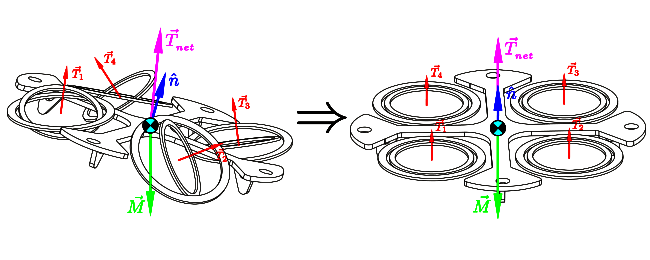
\includegraphics[width=\textwidth]{figs/hover-inertial}
\vspace{-12pt}
\caption{Hover conditions W.R.T the inertial frame $\mathcal{F}^I$}
\label{fig:hover-inertial}
\vspace{-20pt}
\end{figure}
\par
Alternatively, the hover conditions could be defined with respect to the body frame, and being a function of the body's attitude, illustrated in Fig:\ref{fig:hover-body}. The difference is that the body's preferred actuator positions are dependent on each instantaneous orientation. That attitude stays constant whilst the actuators are redirected to produce inertial hovering conditions, irrespective of the attitude. The preferred hovering conditions are then always dependent on the commanded attitude trajectory.
\begin{subequations}\label{eq:hover-body}
\begin{equation}
m_b\vec{G}_b\triangleq m_b Q_b^*\otimes\vec{G}_I\otimes Q_b~~~~\in\mathcal{F}^{b}
\end{equation}
\vspace{-12pt}
\begin{equation}
\vec{\nu}_H=
\begin{bmatrix}
\vec{F}_p\hspace{3pt}\\
\vec{\tau}_p\hspace{3pt}
\end{bmatrix}
=m_b\begin{bmatrix}
\vec{G}_b\\
\vec{C}_b(\vec{u}) \times \vec{G}_b
\end{bmatrix}~~~~\in\mathcal{F}^b
\end{equation}
\end{subequations}
\par
\begin{figure}[htbp]
\vspace{-12pt}
\centering
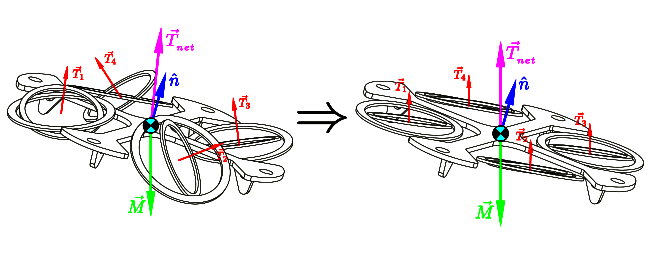
\includegraphics[width=\textwidth]{figs/hover-body}
\vspace{-18pt}
\caption{Hover conditions W.R.T the body frame $\mathcal{F}^b$}
\label{fig:hover-body}
\vspace{-10pt}
\end{figure}
\par
Specific module thrust values to be commanded are then solved for using Eq:\ref{eq:hover} and Eq:\ref{eq:hover-body} with pseudo inversion from Eq:\ref{eq:pseudo-inversion}. The two solutions are then as follows:
\begin{subequations}\label{eq:priority-norm}
\begin{equation}\label{eq:priority-norm-inertial}
\vec{T}_p^I=B^\dagger(\mathbf{x},\vec{\nu}_H\text{}\hspace{-2pt},t)~~\text{for hover in Fig\ref{fig:hover-inertial}}
\end{equation}
\vspace{-15pt}
\begin{equation}\label{eq:priority-norm-body}
\vec{T}_p^b=B^\dagger(\mathbf{x},\vec{\nu}_H,t)~~\text{for hover in Fig:\ref{fig:hover-body}}
\end{equation}
\end{subequations}
Both actuator preferred hovering thrust matrices are then applied to Eq:\ref{eq:inversion} and could potentially be combined with some non-zero weighting matrix, $W\not =\mathbb{I}_{12\times 12}$.
\begin{subequations}
\begin{equation}
\underset{u\in\mathbb{U}}{\vec{T}_{[1:4]}}=(\mathbb{I}_{m\times m}-CB(\vec{\mathbf{x}},t)\big)\vec{T}_p+C\vec{\nu}_d
\end{equation}
\vspace{-10pt}
\begin{equation}
C=W^{-1}B^T(\vec{\mathbf{x}},t)\big(B(\vec{\mathbf{x}},t)W^{-1}B^T(\vec{\mathbf{x}},t)\big)^{-1}
\end{equation}
\end{subequations}
Applying the inverse rotation operator $R^\dagger$ from Eq:\ref{eq:allocator-inersion} to the above, solves for propeller speeds and servo rotational positions in both respective cases. The physical consequences of either preferred hovering condition and its associated actuator positions are demonstrated in simulation in Sec:\ref{sec:simulation.allocator}. Priority actuator positions are not tested together with weighting matrices, the two are compared independently.
%====================================================
\subsection{Weighted Pseudo Inverse Allocator}
\label{subsec:allocation.allocators.weightedinverse}
%====================================================
Adding weights to the inversion in Eq:\ref{eq:inversion}, but regarding preferred actuator positions as negligible, or that $\vec{T}_p=\vec{0}$, produces a \emph{weighted pseudo inverse} allocator. Each weight in $W$ biases a particular actuator's action in $u$, the positive symmetrical weighting matrix is square with respect to the actuator dimension here $W\in\mathbb{R}^{12\times 12}$, but more generally $W\in\mathbb{R}^{m\times m}$. The Moore-Penrose inversion (Eq:\ref{eq:pseudo-inversion}) assumes that each actuator is weighted equally. Such a case makes the weighting matrix $W$ diagonal identity matrix $W = \mathbb{I}_{m\times m}$. 
\par
A weighting matrix could change adaptively over time or as a result of state dependency following control faults or actuator deterioration. As long as the allocator block still produced an actuator command which met the control requirements and any actuator response dynamics where modelled, a changing allocation weight would not affect stability. The control objective of a weighted inversion is to design the explicit weighting coefficients as per some preferred heuristic or optimization. Adaptive weighting is not considered or discussed as that is out of the scope for this work and pertains more to fault tolerant control \cite{FTCallocation}.
\par
Each coefficient in $W$ determines how the least squares solution to Eq:\ref{eq:allocation-problem} preferentially biases a particular thrust vector's component. Multiplication by the weighting matrix $W$ in the quadratic allocation cost function Eq:\ref{eq:allocation-quadratic} increases the cost of a coefficient weighted actuator. Introduction of an inverted weighting matrix in the least squares solution then combines thrust vector components of the produced allocated input $\vec{T}_{[1:4]}$ to produce the control input $\vec{\nu}_d$. 
\begin{figure}[htbp]
\vspace{-6pt}
\centering
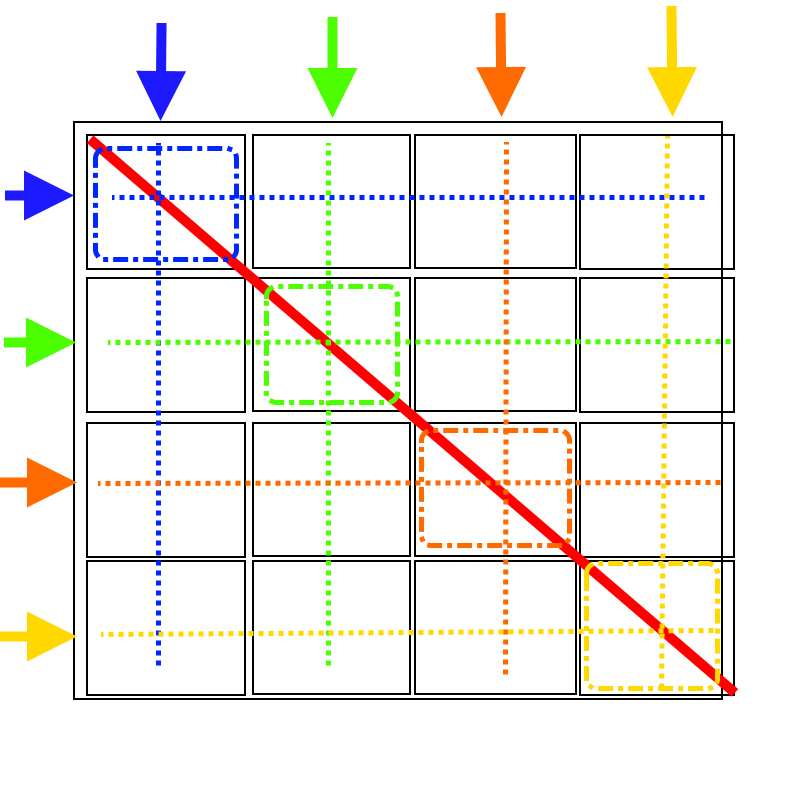
\includegraphics[width=0.6\textwidth]{figs/weighted-matrix}
\vspace{-6pt}
\caption{Weighting matrix biasing}
\label{fig:weighted-matrix-allocation}
\vspace{-6pt}
\end{figure}
\par
Fig:\ref{fig:weighted-matrix-allocation} groups diagonal $[3\times 3]$ weighting coefficients $W_{1\rightarrow 4}$ which relate to individual thrust vector direction biasing ($T_{ix},T_{iy},T_{iz}$), whilst off-centre $[3\times 3]$ groupings mix separate thrust terms $\vec{T}_{1\rightarrow 4}$. 
\par
Pseudo-inversion exactly matches the virtual control input $\vec{\nu}_d=B(\mathbf{x},u_c,t)=\vec{\nu}_c$~so long as the actuators are not saturated and their inputs act sufficiently fast. Biasing actuators could result in gain being applied to the controller input from the allocation block. Such a case could potentially destabilize the trajectory tracking. Short of processing actuator weights online until a viable solution is found, a constraint on the nature of the weighting matrix needs to be introduced to avoid purposefully imposed control slack. So long as each thrust vector $\vec{T}_{[1:4]}$ has its own coefficient group which has row and column vectors that each sum to $1$, the designed control inputs will be met, namely $\sum (W_{row})=\sum (W_{col}) = 1$. Physically, the resultant thrusts and torque (thrust differentials) would be balanced amongst similarly directed components. 
\par
Priority biases for thrust vector components in the $\hat{X}_{b}$ and $\hat{Y}_{b}$ would, in theory, prioritize using pitch or roll servos, $\lambda_i$ and $\alpha_i$, in lieu of changing the propeller's speed $\Omega_i$. However, given that the actuator effort in Eq:\ref{eq:allocation-quadratic} is quadratically optimized, the weighting matrix's effect is, in practice, going to be diminished. Selection of weighting coefficients needs to be designed as per some heuristic. A suitable objective (used in Sec:\ref{sec:simulation.allocator}) for the allocation block, is aiming to minimize each actuator's transfer rate which attempts to improve the net actuator block's bandwidth. A proposed set of weighting coefficients could then be simulated and penalized from actuator slew rate times together with a slack variable norm to ensure that a control objective is still met:
\begin{equation}\label{eq:actuator-penalty}
Q(\vec{s})=\int_{t_0}^{\infty} \big(a\norm{t_{\nu_d-\nu_c}-1}+b||\vec{s}||\big).dt
\end{equation}
where $t_{\nu_d-\nu_c}$ is a matrix of times taken for each commanded control input component of $\vec{\nu}_c(\vec{u}_c)$ to reach their desired setpoints in $\vec{\nu}_d$. That cost integral is evaluated on the body over simulations of multiple step tests in the attitude and position plant, and iteratively optimized following the combined step tests results. The weighting matrix coefficients aim to reduce the transient time for the actuator block to settle whilst ensuring stability is not compromised with the introduction of a slack penalty cost $||\vec{s}||$. However, actuator rates are more dependent on the rotation inverse $R^\dagger(\vec{\mathbf{x}},t)$ and their associated mechanical transfer functions, so the effect of a weighting matrix introduced to the allocation rule is not expected to be significant when the abstraction layer to an affine effectiveness function is introduced.